\section{恒定电场习题解答}

\begin{enumerate}

\item （1分）在导电媒质中，电荷的体密度为
\[
\rho = \nabla\left(\frac{\varepsilon}{\gamma}\right)\cdot\vec{J}
\]
当导电媒质为均匀媒质时，$\varepsilon$ 和 $\gamma$ 都不随空间位置变化，因此电荷密度为零。另一方面，由定义可知，体电流密度为电荷体密度乘以电荷的运动速度。试解释均匀导电媒质中体电流密度不为零而体电荷密度为零这一“矛盾”。

解答：
均匀导电媒质中，$\varepsilon$、$\gamma$ 为常数，故
\[
\nabla\left(\frac{\varepsilon}{\gamma}\right)=0\implies\rho=0
\]
这表示净体电荷密度为零，并不代表不存在电荷。导体中存在大量可自由移动的正负电荷（如金属中的自由电子和晶格正离子），它们的体密度大小相等、符号相反，叠加后净密度为零。

当外加电场时，正负电荷在电场力作用下定向运动：
正电荷沿电场方向运动，负电荷逆电场方向运动，两者的运动方向相反，但电流方向一致，因此会形成不为零的体电流密度 $\vec{J}$。
整个过程中，正负电荷的体密度始终保持大小相等、符号相反，净体电荷密度仍为零。

因此，“净体电荷密度为零”与“体电流密度不为零”并不矛盾。

\item （4分）球形电容器内半径 $R_1=5\,\text{cm}$，外半径 $R_2=10\,\text{cm}$，内外导体间的非理想电介质的电导率 $\gamma=10^{-9}\,\text{S/m}$，若内外导体间电压 $U_0=1000\,\text{V}$，求内外导体间的 $\varphi$、$\vec{E}$、$\vec{J}$ 和绝缘电阻 $R$。
\begin{center}
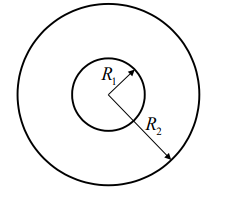
\includegraphics[width=0.3\textwidth]{5.1.png}
\end{center}

解答：
设内导体流出的总电流为 $I$，由对称性，电流密度为径向分布：
\[
\vec{J} = \frac{I}{4\pi r^2}\vec{e}_r,\quad R_1<r<R_2
\]
由欧姆定律 $\vec{J}=\gamma\vec{E}$，得电场：
\[
\vec{E} = \frac{I}{4\pi\gamma r^2}\vec{e}_r
\]
内外导体间电压：
\[
U_0 = \int_{R_1}^{R_2} \vec{E}\cdot d\vec{r} = \frac{I}{4\pi\gamma}\left(\frac{1}{R_1}-\frac{1}{R_2}\right)
\]
解得总电流：
\[
I = \frac{4\pi\gamma U_0 R_1 R_2}{R_2-R_1}
\]

(1) 电场强度：
\[
\vec{E} = \frac{U_0 R_1 R_2}{(R_2-R_1)r^2}\vec{e}_r
\]

(2) 电流密度：
\[
\vec{J} = \gamma\vec{E} = \frac{\gamma U_0 R_1 R_2}{(R_2-R_1)r^2}\vec{e}_r
\]

(3) 电位（以外导体为参考点，$\varphi(R_2)=0$）：
\[
\varphi(r) = \int_r^{R_2} \vec{E}\cdot d\vec{r} = \frac{U_0 R_1 R_2}{R_2-R_1}\left(\frac{1}{r}-\frac{1}{R_2}\right)
\]

(4) 绝缘电阻：
\[
R = \frac{U_0}{I} = \frac{1}{4\pi\gamma}\left(\frac{1}{R_1}-\frac{1}{R_2}\right)
\]
代入数值：
\[
R = \frac{1}{4\pi\times10^{-9}}\left(\frac{1}{0.05}-\frac{1}{0.1}\right) \approx 1.59\times10^9\,\Omega
\]

\item （5分）同轴电缆内导体半径为 $R_1$，外导体半径为 $R_3$，内外导体之间有两层媒质。内层从 $R_1$ 到 $R_2$，媒质的参数为 $\varepsilon_{r1}$ 和 $\gamma_1$；外层从 $R_2$ 到 $R_3$，媒质的参数为 $\varepsilon_{r2}$ 和 $\gamma_2$，如图所示。求：
\begin{enumerate}
    \item 每层单位长度的电容；
    \item 每层单位长度的电导；
    \item 单位长度的总电容；
    \item 单位长度的总电导；
    \item 当同轴电缆长度为 $L$，内外导体之间的电压为 $U$，忽略边缘效应，利用边界上的衔接条件分别求界面 $R_1$、$R_2$ 和 $R_3$ 上的电荷面密度。
\end{enumerate}
\begin{center}
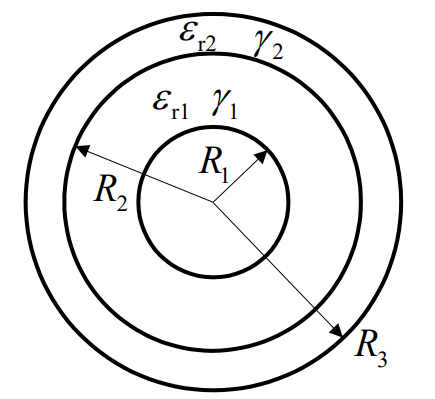
\includegraphics[width=0.3\textwidth]{5.2.png}
\end{center}

解答：
设单位长度电荷为 $\tau$，单位长度漏电流为 $I_0$。

(1) 单位长度电容：
内层（$R_1\sim R_2$）：
\[
C_{01} = \frac{2\pi\varepsilon_1}{\ln(R_2/R_1)},\quad \varepsilon_1=\varepsilon_0\varepsilon_{r1}
\]
外层（$R_2\sim R_3$）：
\[
C_{02} = \frac{2\pi\varepsilon_2}{\ln(R_3/R_2)},\quad \varepsilon_2=\varepsilon_0\varepsilon_{r2}
\]

(2) 单位长度电导：
内层（$R_1\sim R_2$）：
\[
G_{01} = \frac{2\pi\gamma_1}{\ln(R_2/R_1)}
\]
外层（$R_2\sim R_3$）：
\[
G_{02} = \frac{2\pi\gamma_2}{\ln(R_3/R_2)}
\]

(3) 单位长度总电容（两层串联）：
\[
\frac{1}{C_0} = \frac{1}{C_{01}}+\frac{1}{C_{02}} \implies C_0 = \frac{C_{01}C_{02}}{C_{01}+C_{02}}
\]

(4) 单位长度总电导（两层串联）：
\[
frac{1}{G_0} = \frac{1}{G_{01}}+\frac{1}{G_{02}} \implies G_0 = \frac{G_{01}G_{02}}{G_{01}+G_{02}}
\]

(5) 界面电荷面密度：
由电流连续性，两层电流密度法向连续：$J_{1n}=J_{2n}$，即
\[
\gamma_1 E_1 = \gamma_2 E_2 = J_0
\]
电压：
\[
U = E_1\ln\frac{R_2}{R_1} + E_2\ln\frac{R_3}{R_2}
\]
解得：
\[
E_1 = \frac{U\gamma_2}{\gamma_2\ln\frac{R_2}{R_1}+\gamma_1\ln\frac{R_3}{R_2}},\quad E_2 = \frac{U\gamma_1}{\gamma_2\ln\frac{R_2}{R_1}+\gamma_1\ln\frac{R_3}{R_2}}
\]
$R_1$ 处：
\[
\sigma_1 = \varepsilon_1 E_1 = \frac{\varepsilon_1 U\gamma_2}{\gamma_2\ln\frac{R_2}{R_1}+\gamma_1\ln\frac{R_3}{R_2}}
\]
$R_2$ 处：
\[
\sigma_2 = \varepsilon_2 E_2 - \varepsilon_1 E_1 = \frac{U(\varepsilon_2\gamma_1-\varepsilon_1\gamma_2)}{\gamma_2\ln\frac{R_2}{R_1}+\gamma_1\ln\frac{R_3}{R_2}}
\]
$R_3$ 处：
\[
\sigma_3 = -\varepsilon_2 E_2 = -\frac{\varepsilon_2 U\gamma_1}{\gamma_2\ln\frac{R_2}{R_1}+\gamma_1\ln\frac{R_3}{R_2}}
\]

\item （1分）假设大地为均匀导电媒质，浅埋于地下的不规则形状接地体电流流入大地。在远离接地体的大地内，电流如何分布？

解答：
在远离接地体的区域，接地体可近似看作点电流源，电流以径向对称的方式向四周扩散。

电流密度分布为：
\[
\vec{J} = \frac{I}{2\pi r^2}\vec{e}_r
\]
对应的电场强度为：
\[
\vec{E} = \frac{\vec{J}}{\gamma} = \frac{I}{2\pi\gamma r^2}\vec{e}_r
\]
电流呈球面辐射状分布，且随着距离 $r$ 的增大，电流密度按 $1/r^2$ 规律衰减。

\item （3分）图示平行平板电容器，两极板间距为 $d$，极板之间有两种电介质，第一种电介质厚度为 $a$，介电常数为 $\varepsilon_1$，电导率为 $\gamma_1$；第二种电介质厚度为 $d-a$，介电常数为 $\varepsilon_2$，电导率为 $\gamma_2$。若两极板间加电压 $U$，求电介质中的电场强度、漏电流密度和电介质分界面上的自由电荷面密度。
\begin{center}
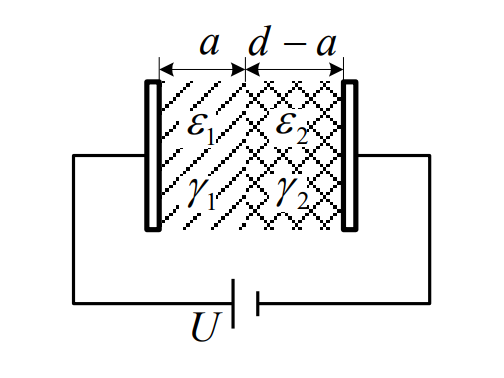
\includegraphics[width=0.4\textwidth]{5.3.png}
\end{center}

解答：
由电流连续性，两种介质中漏电流密度相等，设为 $J$，则：
\[
E_1 = \frac{J}{\gamma_1},\quad E_2 = \frac{J}{\gamma_2}
\]
电压关系：
\[
U = E_1 a + E_2 (d-a) = J\left(\frac{a}{\gamma_1}+\frac{d-a}{\gamma_2}\right)
\]
解得：
\[
J = \frac{U\gamma_1\gamma_2}{\gamma_2 a + \gamma_1(d-a)}
\]

(1) 电场强度：
\[
E_1 = \frac{U\gamma_2}{\gamma_2 a + \gamma_1(d-a)},\quad E_2 = \frac{U\gamma_1}{\gamma_2 a + \gamma_1(d-a)}
\]

(2) 漏电流密度：
\[
J = \frac{U\gamma_1\gamma_2}{\gamma_2 a + \gamma_1(d-a)}
\]

(3) 分界面自由电荷面密度：
\[
\sigma = \varepsilon_2 E_2 - \varepsilon_1 E_1 = \frac{U(\varepsilon_2\gamma_1-\varepsilon_1\gamma_2)}{\gamma_2 a + \gamma_1(d-a)}
\]

\item （2分）在恒定电场的电源中，总的电场强度闭合线积分为零吗？局外电场强度的闭合线积分为零吗？库仑电场强度的闭合线积分为零吗？在电源之外，上述3个闭合线积分是否为零？

解答：
设电源内的总电场为 $\vec{E}=\vec{E}_c+\vec{E}_e$，其中 $\vec{E}_c$ 为库仑电场，$\vec{E}_e$ 为局外电场。

电源内部：
总电场：$\oint \vec{E}\cdot d\vec{l} = \oint (\vec{E}_c+\vec{E}_e)\cdot d\vec{l} \neq 0$
局外电场：$\oint \vec{E}_e\cdot d\vec{l} \neq 0$
库仑电场：$\oint \vec{E}_c\cdot d\vec{l} = 0$

电源外部：
局外电场 $\vec{E}_e=0$，总电场等于库仑电场，因此：
\[
\oint \vec{E}\cdot d\vec{l} = \oint \vec{E}_c\cdot d\vec{l} = 0
\]
三个积分均为零。

\item （2分）请依据电流密度矢量 $\vec{J}$ 的定义及电流连续性定理，分别给出电路理论中焦耳定律（微分形式）与基尔霍夫电流定律的推导过程。

解答：
焦耳定律（微分形式）推导：
单位体积内的功率损耗（焦耳热）等于电场力对电荷做功的功率。
由欧姆定律 $\vec{J}=\gamma\vec{E}$，单位体积功率：
\[
p = \vec{J}\cdot\vec{E} = \gamma E^2
\]
即焦耳定律的微分形式：$p=\vec{J}\cdot\vec{E}$。

基尔霍夫电流定律（KCL）推导：
电流连续性定理：
\[
\nabla\cdot\vec{J} = -\frac{\partial\rho}{\partial t}
\]
恒定电流下 $\frac{\partial\rho}{\partial t}=0$，故 $\nabla\cdot\vec{J}=0$。
对节点取闭合面，由高斯定理：
\[
\oiint_S \vec{J}\cdot d\vec{S} = 0
\]
即流入节点的电流之和等于流出节点的电流之和，对应KCL：
\[
\sum I_k = 0
\]

\end{enumerate}